\documentclass[12pt]{amsart}
\usepackage{amsmath,amssymb,amsthm,bm}
\usepackage[usenames,dvipsnames]{xcolor}
\usepackage{graphicx}
%\usepackage{lmodern}
\usepackage[T1]{fontenc}
%\usepackage{textcomp}
\usepackage{pxfonts}
\usepackage{enumerate,verbatim,cite}
\usepackage[margin=1in]{geometry}
%\usepackage{../../tex/pythonhighlight} %https://github.com/olivierverdier/python-latex-highlighting
\usepackage[framed]{mcode}

\usepackage{fancyhdr}
\pagestyle{fancy}
%\addtolength{\headheight}{\baselineskip}
\addtolength{\footskip}{\baselineskip}
\renewcommand{\headrulewidth}{0pt}
\renewcommand{\footrulewidth}{0.4pt}
\fancyhf{}
\fancyfoot[L]{\textit{Last Modified: \today}}
\fancyfoot[C]{\thepage}


\usepackage[pdftex,bookmarks,hyperfigures,colorlinks
						,urlcolor=blue
						,citecolor=blue
						,linkcolor=blue
						,pdfstartview=FitH]{hyperref}


%\usepackage{epsf}
% \topmargin -0.5in \setlength{\textwidth}{6.in}
% \setlength{\textheight}{8.5in}
%\setlength{\evensidemargin}{0.25in}
% \setlength{\oddsidemargin}{0.25in}
\renewcommand{\r}{{\bf r}}
\newcommand{\dery}{\frac{dx}{dt}}
\renewcommand{\k}{{\bf k}}
\newcommand{\be}{\begin{equation}}
\newcommand{\ee}{\end{equation}}
%\usepackage[usenames,dvipsnames]{xcolor}
%\usepackage{hyperref}


\title{Applied Math 50 Lab 2: Imaging\\
Matrices, images, and the Radon transform
}

\date{}

\begin{document}
\maketitle

\section{Introduction}
Today's computer lab has two aims:
\begin{enumerate}
	\item Learn how to generate, import, and manipulate images (matrices) in Matlab
	\item Explore the Radon transform and applications to medical image reconstruction.
\end{enumerate}

\section{Getting started with images}

\noindent We'll begin this lab by discussing how to handle images in Matlab.  Matlab has good support for manipulating images via the image processing toolbox.  To find out of this toolbox is installed on your computer, type \verb+ ver+ at the prompt in the command window and hit enter.  Scroll through the list and make sure that you see ``Image Processing Toolbox.''  If you do, then you're ready to get started.  \\

\noindent  As we briefly described in class 8, an image can be represented as a matrix.  For grayscale image, the entries $v_{ij}$ of the matrix represent the pixel intensity, with $v_{ij} = 1$ corresponding to white, $v_{ij} = 0$ corresponding to black, and $0 < v_{ij} < 1$ corresponding to various shades of gray.    Let's examine the code for the simple 81 pixel image generated by the script file below.  

\bigskip

\begin{center}
\colorbox{Goldenrod}{\parbox{15cm}{
{
\textbf{\large Exercise 1}\vspace{1mm} \\
Read through the code.  On paper, carefully draw the 81 pixel image according to the commands defined in the script.  }}}
\end{center}
\bigskip


\lstinputlisting{SimpleImage.m}
\smallskip


\noindent Type the script into Matlab and save it as \verb+SimpleImage.m+.  Run the script and compare the output to your sketch in Exercise 1.  If your sketch doesn't agree with the Matlab output, go back to your sketch to reconcile the differences.  \\

\smallskip \noindent Now let's create the 200 x 200 pixel images below.  
\begin{center}
  %\begin{longtable}{cc}
  
\includegraphics[width=.4\textwidth]{bigsimpleimage} 
    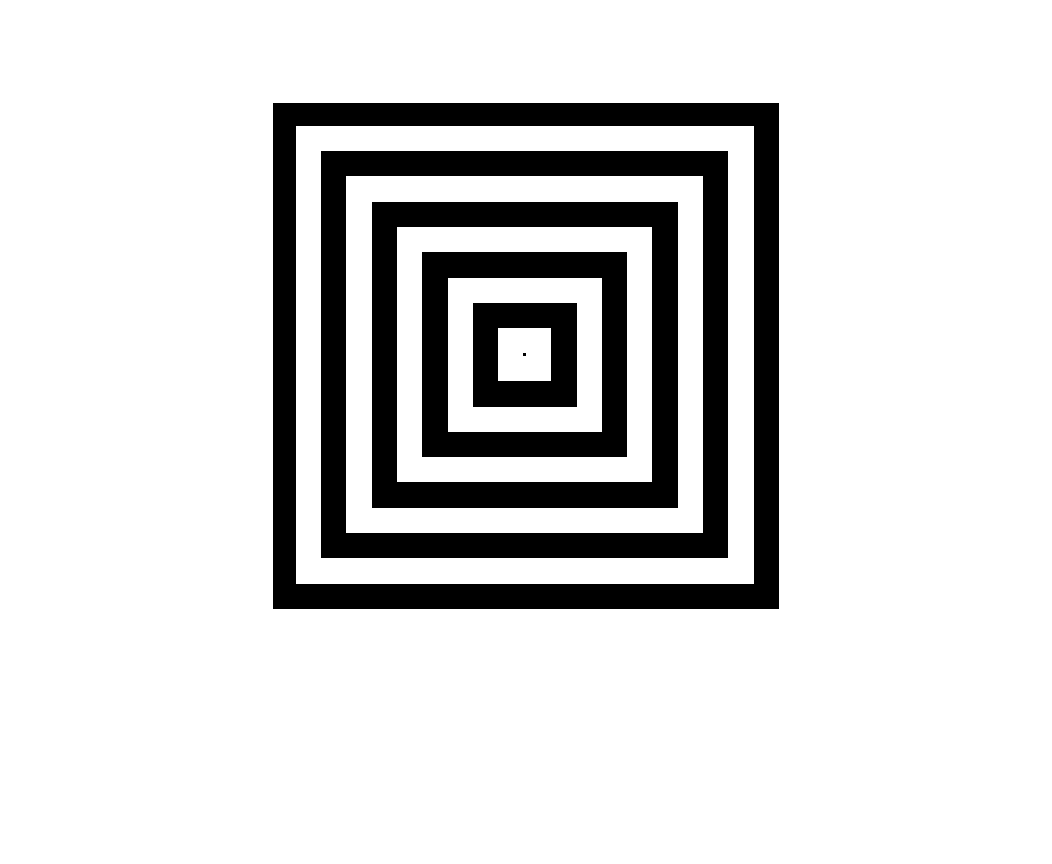
\includegraphics[width=0.4\textwidth]{bigsimpleimage2} 
\end{center}
\vspace{-.5in}

\noindent Open and save a new script called \verb+BigSimpleImage.m+ and make a 200 x 200 black image.  Then write and save a new function called \verb+makesquare.m+, according the instructions in the exercise 2 below.

\bigskip

\begin{center}
\colorbox{Goldenrod}{\parbox{15cm}{
{
\textbf{\large Exercise 2}\vspace{1mm} \\
Write a function that takes in an image and outputs the same image with a square of a specified shade (black or white).  The function should have six inputs: the image, the coordinates of the pixel that corresponds to the upper left corner of the square, the dimensions of the square, and the shade of the square.  }}}
\end{center}
\bigskip
\begin{center}
\colorbox{Goldenrod}{\parbox{15cm}{
{
\textbf{\large Exercise 3}\vspace{1mm} \\
Call your function several times in BigSimpleImage.m to create the leftmost image above.   Then modify your script to make the rightmost image.   For the rightmost image, you may want to use a loop as well as the Matlab function mod.}}}
\end{center}

\section{Color images and real images}

\noindent Color images can be created by using three separate channels for the red, green, and blue components.  To represent an image of $M$ rows and $N$ columns in Matlab, a three dimensional array \verb+V+ of size $ M \times N \times 3$ can be created with \verb+V(i, j, 1)+, \verb+V(i, j, 2)+, and \verb+V(i, j, 3)+ representing the red, green, and blue channel values, respectively.  An arbitrary color can be made by combining these three components.  
\bigskip
\begin{center}
\colorbox{Goldenrod}{\parbox{15cm}{
{
\textbf{\large Exercise 4}\vspace{1mm} \\
Modify the script from exercise 1 to make a color image with blue eyes, red nose, and orange mouth.  See \url{https://www.w3schools.com/colors/colors_rgb.asp} for tips on making different colors.}}}
\end{center}
\bigskip
\noindent Now let's play around with a real image.  To do this we first need a real image to import into Matlab.  Go to my.harvard and download and save your house photo as a headshot.jpg in your working directory.  In the command window, type the following:  
\bigskip
\begin{verbatim}
clear all;
I = imread('headshot.jpg');
save I
\end{verbatim}
\bigskip

\noindent The Matlab command \verb+imread+ reads in headshot.jpg and stores it in the matrix \verb+I+.  Then command \verb+save+ saves the matrix \verb+I+ as \verb+I.mat+.  If you type \verb+ls+ in your command window, all the files in your working directory are listed.  You should see the file \verb+I.mat+ which contains the variable \verb+I+.  Now open and save a new script \verb+MyHousePhoto.m+ with the following lines of code:


\lstinputlisting{MyHousePhoto.m}
\smallskip

\noindent The command \verb+Ibw = im2double(Ibw)+ converts every entry in the image matrix from ``unsigned 8-bit integer'' to ``double.''  If you're not familiar with these data types, don't worry about it.  Images tend to be very large and require a lot of computer memory for storage, and storing images as unsigned 8-bit integer (uint8) saves space.    But Matlab doesn't like to operate on uint8 matrices, so we need to first convert the entries of the image matrix to a format that Matlab likes, ie, double.  You can then modify the image in whatever way you like and save it by first converting back to uint8 with the command \verb+im2uint8+.

\bigskip
\begin{center}
\colorbox{Goldenrod}{\parbox{15cm}{
{
\textbf{\large Exercise 5}\vspace{1mm} \\
Crop your house photo and make a new color image with only your eyes.  You can crop an image by estimating the coordinates the region of interest, or you can use a Matlab function called imcrop.  Then modify the image so that your left eye is on the right hand side of the image and your right eye is on the left hand side.  }}}
\end{center}

\section{Transforms and image reconstruction}

\noindent Last week in class we discussed inverse problems, particularly in the context of radiology and CT-scans.  Suppose we're given a data set and we're told that it contains information about an image.  Can we recover the image from this data?  A CT scanner acquires data about the attenuation distribution of the materials in your body.  Then -- without cutting you open! -- a computer reconstructs an image of your insides by processing the data in a special way, ie, by inverting the Radon transform.  We'll explore this with a simple image.  Make a new script called \verb+ImageRecon.m+ and create a 128 x 128 image with an 32 x 32 white square in the center of the image.  The square represents you, about to undergo a CT scan.  The command \\

\verb+sinogram =  radon(image, angles)+ \\

\noindent takes the Radon transform of the image at given angles with respect to the horizontal.  We began talking about this magical transform in class, and we'll continue to work with it on next week's homework.   The important point is that a CT scanner essentially measures the Radon transform of you, taken from various views around your body.  For example, \verb+sinogram =  radon(image, 0:180:360)+ takes the Radon transform of the image matrix at $\theta = 0, 180, 360$ degrees.  Add this command to your script.  Then run the script and notice the size of the variable \verb+sinogram+.  The first column is the Radon transform ``shadow'' of the image taken along horizontal lines.  This shadow is often called a projection.  The second column is also a projection, this time taken along lines that form 180$^o$ angles with respect to the horizontal.  The third column is the projection along lines that form 360$^o$ angles with respect to the horizontal.  And so on.
\bigskip
\begin{center}
\colorbox{Goldenrod}{\parbox{15cm}{
{
\textbf{\large Exercise 6}\vspace{1mm} \\
Use the Matlab function subplot to plot the first, second, and third columns of sinogram on one figure but in three separate plots.    Do these projections make sense given what you know about you?  (Remember that for the purposes of this exercise, you are a square.)\\ 
 }}}
\end{center}


\bigskip
\noindent You can get the projections at many more angles by modifying the angle argument in \verb+radon+.  Modify the command in your script  to calculate the Radon transform at $\theta = 0, 4, 8, \ldots, 360$.  

\bigskip
\begin{center}
\colorbox{Goldenrod}{\parbox{15cm}{
{
\textbf{\large Exercise 7}\vspace{1mm} 
\\ 
Since you are an object with symmetry, you might suspect that some of your projections are identical.  When two projections are identical, we say that they are redundant.  Determine which projections are redundant.  }}}
\end{center}

\bigskip

\noindent Now given that you only know the projections (\verb+sinogram+ in your code) from the scanner, how do we reconstruct your original image of your insides (\verb+image+ in your code)?  The command \\

\verb+imagerecon = iradon(sinogram, angles)+ \\

\noindent inverts the Radon transform to recover the original image!

\bigskip
\begin{center}
\colorbox{Goldenrod}{\parbox{15cm}{
{
\textbf{\large Exercise 8}\vspace{1mm} 
\\ 
Modify your script to compute the Radon transform only at $\theta = 0, 180, 360$.  Then use iradon to invert the transform.  Use subplot to make a figure with two images: the original image and the reconstructed image.   Does your reconstructed image look like the original image?  What goes wrong?  Try:\\
\begin{enumerate}
\item Using more angles:  calculate the Radon transform at $\theta = 0, 4, 8, \ldots, 360$.  Plot the original image and the reconstructed image.
\item Using more angles but only between $\theta = 0$ and $\theta = 180$.  Calculate the Radon transform at $\theta = 0, 1, 2, \ldots, 180$.  Plot the original image and the reconstructed image.  Does the reconstructed image look better, worse, or the same as the reconstructed image in (1)?
\end{enumerate}
 }}}
\end{center}



\end{document}
